\section{Comparison}
\label{sec:comparison}

% STDP-like paper
The \ac{SNN} model from \cite{STDP_like} determines its output by 
choosing the class of the first neuron pool to reach the descision threshold with its accumulated sensory evidence.
The authors claim that the original method of using a majority vote of single threshold-based neuron acticity is less biologically plausible.

Not only the \cite{STDP_like} model but also the \cite{SNN} model use inhibition.

The authors of \cite{STDP_like} point out that the classifier neuron will not recognize atypical digits (i.e. their stimulus).
Therefore, the ability to generalize on new datasets depends on the inputs' similiarity to the learned patterns.

% original paper
The authors of \cite{SNN} 

\textcolor{red}{to other implementations, to biology}

% DIET-SNN paper
% Captial L to avoid strange behaviour since figure is close to page break
\begin{wrapfigure}{L}{0.1\textwidth}
    \centering
    \vspace{-20pt}
    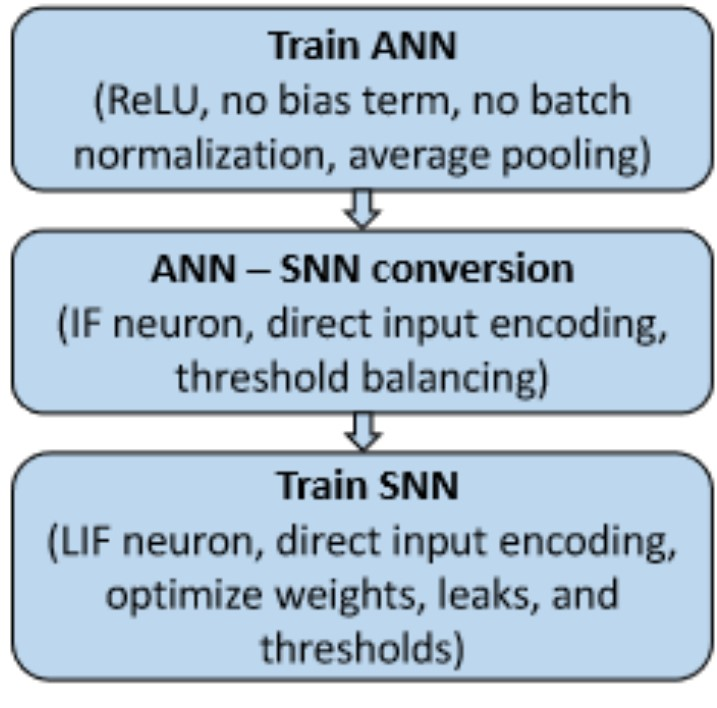
\includegraphics[width=0.1\textwidth]{pictures/DIET_SNN_pipeline.jpg}
    \caption{\ac{DIET}-\ac{SNN} training pipeline from \cite{DIET_SNN}}
    \label{fig:training_pipeline_DIET_SNN}
\end{wrapfigure}

The \ac{DIET}-\ac{SNN} model from \cite{DIET_SNN} is an entriely different approach to those discussed before.
As depicted in \autoref{fig:training_pipeline_DIET_SNN}, an \ac{ANN} is trained and thereafter converted into a \ac{SNN}.
The initialized parameters speed up the subsequent training wit spike-based backpropagation.
Instead of using a Poisson generator (rate-coding: converting analog values to spike-train),the image pixels are directly applied as input.
The first convolutional layer is trained to encode them as spikes.